\documentclass{article}
\usepackage{graphicx}

\title{Encoding Schemes}
\author{William Y. Feng}

\begin{document}

\maketitle
\textit{Encoding} (infinitive: to encode) is the process of turning one form of data into another form of data. This is quite a vague definition, so in this article, I'll be giving some examples to clarify what it means!

Side note: Perhaps you've heard of the similar but subtly different term \textbf{encryption}, which describes the process of encoding data such that it is only readable to certain people who have the proper keys, and unreadable to everyone else. Encoding doesn't mix up data like that; its purpose is to describe ways to work with data so that anyone, regardless of what piece of technology they're using or where they are in the world, can communicate with anyone else.

Now let's dive into some concrete examples.

\textbf{ASCII:}
The American Standard Code for Information Interchange (ASCII) is a widely-known \textbf{encoding scheme} that assigns an integer (known as a \textbf{code point}) to every English letter (uppercase and lowercase), punctuation mark, and digit, among other characters.

For instance, the uppercase letter ``A" is encoded as 65 under ASCII, and the lowercase letter ``a" is encoded 97. The digit ``0" is 48, and the exclamation mark is 33. A full table of encodings is shown below:

\begin{center}
    \footnotesize
    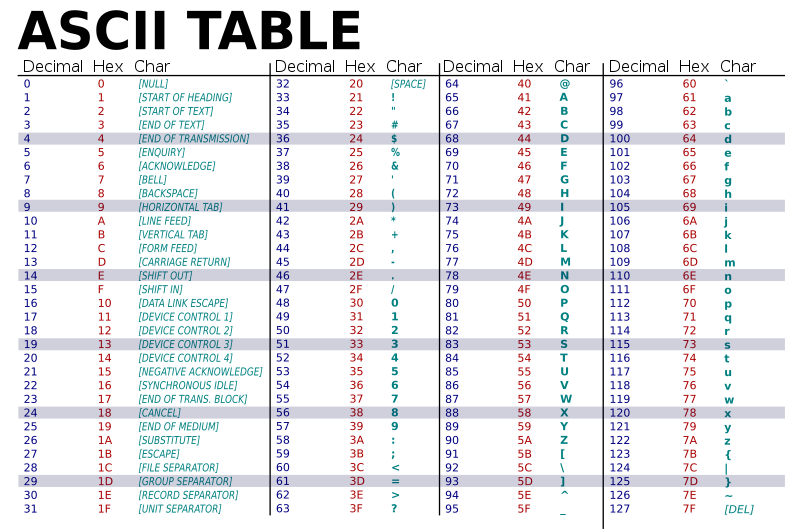
\includegraphics[width = 2 in]{images/ascii_table.png}
    \textit{ASCII table from \url{https://commons.wikimedia.org/wiki/File:ASCII-Table-wide.svg}. Also, if you're curious about the HEX column, read on! We'll be discussing it in a couple paragraphs.}
\end{center}

There is a method to the madness of ASCII. It was initially published over sixty years ago in 1963, so while there do exist some now-obsolete characters, a lot of stuff still makes sense. ASCII can roughly be divided into four ``character sets," represented by the code point ranges 0-31, 32-63, 64-95, and 96-127.
\begin{enumerate}
    \item The first character set includes some antiquated characters like ``device control" and ``record separator," but it also includes stuff that's still used, like ``line feed" (10) and ``horizontal tab" (9).
    \item The second character set includes punctuation, like the space character (32), as well as digits—``0" through ``9" map to code points 48 through 57.
    \item The third character set includes the uppercase letters ``A" through ``Z" as its main chunk, using code points 65 through 90, as well as some punctuation.
    \item The fourth character set includes the lowercase letters ``a" through ``z," which use code points 97 through 122, and some more punctuation.
\end{enumerate}

If we think of these code points in terms in terms of binary, then every code point can be represented as a $7$-bit binary number (that is, a binary number with $7$ digits), since code points range from $0=0000000_2$ to $127=1111111_2$, inclusive. Then these character sets actually make a lot of sense—if the first two bits of the code point are 00, then the corresponding character is in first character set. If the first two bits are 01, then this character is in the second character set. So on and so forth...

Another point of genius in ASCII is that the uppercase letters and lowercase letters are spaced apart by exactly 32: take S, for instance. Its code point is $83$, and if we add $32$ to it, we get $115$, which is the code point for lowercase s.

\textbf{Hex and Binary Stuff:}
Getting a bit deeper into the weeds, we bump into the problem of representing text on computers. ASCII provides a helpful way of turning characters into integers through code point conversions, but we still need a way to represent these integers as bits on a computer.

Thankfully, this is fairly simple: if we turn the code point into a $7$-bit integer, we can store that a computer fairly simply because computers are good at storing binary. Unfortunately, computers usually work in $8$-bit chunks of information called \textbf{bytes}, so every character encoded with ASCII will take up one byte, in which one bit is wasted.

\textbf{Unicode:} 
But not everyone in the world speaks English, and even English words like Beyoncé require accents on characters that ASCII can't represent. This is where \textbf{Unicode} comes in: it's a way of turning even more characters, beyond the basic English alphabet and some punctuation, into code points (again, those are just integers).

Unicode doesn't prescribe any way of turning these code points into computer memory, but there are some fairly common standards like UTF-8 that prety much the whole world has agreed to use.

It often amazes me how the world has managed to stick to a standard set of encodings so that technology across the world can communicate seamlessly. The history of encoding is an endlessly fascinating topic, rich with history and brimming with ingenuity, and there's no way we can cover all that in a single article. Hopefully, though, I've explained enough about ASCII in this article so that the next time someone sends you a secret message encoded in ones and zeros, you'll know what's really going on :)

If you're interested in diving deeper into this topic, there's an excellent article by Joel Spolsky titled ``The Absolute Minimum Every Software Developer Absolutely, Positively Must Know About Unicode and Character Sets (No Excuses!)" that you should check out: \url{https://www.joelonsoftware.com/2003/10/08/the-absolute-minimum-every-software-developer-absolutely-positively-must-know-about-unicode-and-character-sets-no-excuses}
\end{document}